\documentclass[twoside]{book}

% Packages required by doxygen
\usepackage{fixltx2e}
\usepackage{calc}
\usepackage{doxygen}
\usepackage[export]{adjustbox} % also loads graphicx
\usepackage{graphicx}
\usepackage[utf8]{inputenc}
\usepackage{makeidx}
\usepackage{multicol}
\usepackage{multirow}
\PassOptionsToPackage{warn}{textcomp}
\usepackage{textcomp}
\usepackage[nointegrals]{wasysym}
\usepackage[table]{xcolor}

% NLS support packages
\usepackage[french]{babel}

% Font selection
\usepackage[T1]{fontenc}
\usepackage[scaled=.90]{helvet}
\usepackage{courier}
\usepackage{amssymb}
\usepackage{sectsty}
\renewcommand{\familydefault}{\sfdefault}
\allsectionsfont{%
  \fontseries{bc}\selectfont%
  \color{darkgray}%
}
\renewcommand{\DoxyLabelFont}{%
  \fontseries{bc}\selectfont%
  \color{darkgray}%
}
\newcommand{\+}{\discretionary{\mbox{\scriptsize$\hookleftarrow$}}{}{}}

% Page & text layout
\usepackage{geometry}
\geometry{%
  a4paper,%
  top=2.5cm,%
  bottom=2.5cm,%
  left=2.5cm,%
  right=2.5cm%
}
\tolerance=750
\hfuzz=15pt
\hbadness=750
\setlength{\emergencystretch}{15pt}
\setlength{\parindent}{0cm}
\setlength{\parskip}{3ex plus 2ex minus 2ex}
\makeatletter
\renewcommand{\paragraph}{%
  \@startsection{paragraph}{4}{0ex}{-1.0ex}{1.0ex}{%
    \normalfont\normalsize\bfseries\SS@parafont%
  }%
}
\renewcommand{\subparagraph}{%
  \@startsection{subparagraph}{5}{0ex}{-1.0ex}{1.0ex}{%
    \normalfont\normalsize\bfseries\SS@subparafont%
  }%
}
\makeatother

% Headers & footers
\usepackage{fancyhdr}
\pagestyle{fancyplain}
\fancyhead[LE]{\fancyplain{}{\bfseries\thepage}}
\fancyhead[CE]{\fancyplain{}{}}
\fancyhead[RE]{\fancyplain{}{\bfseries\leftmark}}
\fancyhead[LO]{\fancyplain{}{\bfseries\rightmark}}
\fancyhead[CO]{\fancyplain{}{}}
\fancyhead[RO]{\fancyplain{}{\bfseries\thepage}}
\fancyfoot[LE]{\fancyplain{}{}}
\fancyfoot[CE]{\fancyplain{}{}}
\fancyfoot[RE]{\fancyplain{}{\bfseries\scriptsize Généré par Doxygen }}
\fancyfoot[LO]{\fancyplain{}{\bfseries\scriptsize Généré par Doxygen }}
\fancyfoot[CO]{\fancyplain{}{}}
\fancyfoot[RO]{\fancyplain{}{}}
\renewcommand{\footrulewidth}{0.4pt}
\renewcommand{\chaptermark}[1]{%
  \markboth{#1}{}%
}
\renewcommand{\sectionmark}[1]{%
  \markright{\thesection\ #1}%
}

% Indices & bibliography
\usepackage{natbib}
\usepackage[titles]{tocloft}
\setcounter{tocdepth}{3}
\setcounter{secnumdepth}{5}
\makeindex

% Hyperlinks (required, but should be loaded last)
\usepackage{ifpdf}
\ifpdf
  \usepackage[pdftex,pagebackref=true]{hyperref}
\else
  \usepackage[ps2pdf,pagebackref=true]{hyperref}
\fi
\hypersetup{%
  colorlinks=true,%
  linkcolor=blue,%
  citecolor=blue,%
  unicode%
}

% Custom commands
\newcommand{\clearemptydoublepage}{%
  \newpage{\pagestyle{empty}\cleardoublepage}%
}

\usepackage{caption}
\captionsetup{labelsep=space,justification=centering,font={bf},singlelinecheck=off,skip=4pt,position=top}

%===== C O N T E N T S =====

\begin{document}

% Titlepage & ToC
\hypersetup{pageanchor=false,
             bookmarksnumbered=true,
             pdfencoding=unicode
            }
\pagenumbering{alph}
\begin{titlepage}
\vspace*{7cm}
\begin{center}%
{\Large Compresseur / Décompresseur de Huffman \\[1ex]\large 1.\+1 }\\
\vspace*{1cm}
{\large Généré par Doxygen 1.8.13}\\
\end{center}
\end{titlepage}
\clearemptydoublepage
\pagenumbering{roman}
\tableofcontents
\clearemptydoublepage
\pagenumbering{arabic}
\hypersetup{pageanchor=true}

%--- Begin generated contents ---
\chapter{Index des classes}
\section{Liste des classes}
Liste des classes, structures, unions et interfaces avec une brève description \+:\begin{DoxyCompactList}
\item\contentsline{section}{\hyperlink{structCode}{Code} \\*Codage d\textquotesingle{}un charactère }{\pageref{structCode}}{}
\item\contentsline{section}{\hyperlink{structNoeud}{Noeud} \\*\hyperlink{structNoeud}{Noeud} de l\textquotesingle{}arbre d\textquotesingle{}Huffman }{\pageref{structNoeud}}{}
\end{DoxyCompactList}

\chapter{Index des fichiers}
\section{Liste des fichiers}
Liste de tous les fichiers documentés avec une brève description \+:\begin{DoxyCompactList}
\item\contentsline{section}{\hyperlink{compress_8h}{compress.\+h} \\*Fonction de compilation Huffman }{\pageref{compress_8h}}{}
\item\contentsline{section}{\hyperlink{decompress_8h}{decompress.\+h} \\*Fonction de décompilation Huffman }{\pageref{decompress_8h}}{}
\item\contentsline{section}{\hyperlink{header_8h}{header.\+h} \\*Fonction de Création d\textquotesingle{}index Huffman }{\pageref{header_8h}}{}
\item\contentsline{section}{\hyperlink{main_8c}{main.\+c} \\*Programme de Création d\textquotesingle{}index, compilation et décompilation Huffman }{\pageref{main_8c}}{}
\end{DoxyCompactList}

\chapter{Documentation des classes}
\hypertarget{structCode}{}\section{Référence de la structure Code}
\label{structCode}\index{Code@{Code}}


{\ttfamily \#include $<$header.\+h$>$}

\subsection*{Attributs publics}
\begin{DoxyCompactItemize}
\item 
int \hyperlink{structCode_a2a982a26130ccdf0c62a00b39bad7f15}{bit}
\item 
\mbox{\Hypertarget{structCode_a8f7398fe11db54f06d78147978f75a13}\label{structCode_a8f7398fe11db54f06d78147978f75a13}} 
unsigned char $\ast$ {\bfseries code}
\end{DoxyCompactItemize}


\subsection{Description détaillée}
bit est le nombre de bit du code. code est le code. 

\subsection{Documentation des données membres}
\mbox{\Hypertarget{structCode_a2a982a26130ccdf0c62a00b39bad7f15}\label{structCode_a2a982a26130ccdf0c62a00b39bad7f15}} 
\index{Code@{Code}!bit@{bit}}
\index{bit@{bit}!Code@{Code}}
\subsubsection{\texorpdfstring{bit}{bit}}
{\footnotesize\ttfamily int Code\+::bit}

bit != (byte$\vert$$\vert$octet) 

La documentation de cette structure a été générée à partir du fichier suivant \+:\begin{DoxyCompactItemize}
\item 
\hyperlink{header_8h}{header.\+h}\end{DoxyCompactItemize}

\hypertarget{structNoeud}{}\section{Référence de la structure Noeud}
\label{structNoeud}\index{Noeud@{Noeud}}


{\ttfamily \#include $<$header.\+h$>$}

\subsection*{Attributs publics}
\begin{DoxyCompactItemize}
\item 
\mbox{\Hypertarget{structNoeud_a2ea9146a5bd3678a27f8a56c9306de22}\label{structNoeud_a2ea9146a5bd3678a27f8a56c9306de22}} 
int {\bfseries pere}
\item 
\mbox{\Hypertarget{structNoeud_a2aeffae918ba8274b8b5f75706bb84de}\label{structNoeud_a2aeffae918ba8274b8b5f75706bb84de}} 
int {\bfseries fg}
\item 
\mbox{\Hypertarget{structNoeud_a67400f9553fd71df5a67cf32dc2ab639}\label{structNoeud_a67400f9553fd71df5a67cf32dc2ab639}} 
int {\bfseries fd}
\item 
\mbox{\Hypertarget{structNoeud_a2678aa0eb590d87e8b61d071c2d5b995}\label{structNoeud_a2678aa0eb590d87e8b61d071c2d5b995}} 
double {\bfseries freq}
\end{DoxyCompactItemize}


\subsection{Description détaillée}
pere est le père du \hyperlink{structNoeud}{Noeud}. fg est le fils gauche du \hyperlink{structNoeud}{Noeud}. fd est le fils droit du \hyperlink{structNoeud}{Noeud}. freq est le poid du noeud. Le poid peut être négligé dans certaine condition d\textquotesingle{}utilisation comme la décompression. 

La documentation de cette structure a été générée à partir du fichier suivant \+:\begin{DoxyCompactItemize}
\item 
\hyperlink{header_8h}{header.\+h}\end{DoxyCompactItemize}

\chapter{Documentation des fichiers}
\hypertarget{compress_8h}{}\section{Référence du fichier compress.\+h}
\label{compress_8h}\index{compress.\+h@{compress.\+h}}
{\ttfamily \#include $<$stdio.\+h$>$}\newline
{\ttfamily \#include $<$stdlib.\+h$>$}\newline
{\ttfamily \#include \char`\"{}header.\+h\char`\"{}}\newline
Graphe des dépendances par inclusion de compress.\+h\+:
\nopagebreak
\begin{figure}[H]
\begin{center}
\leavevmode
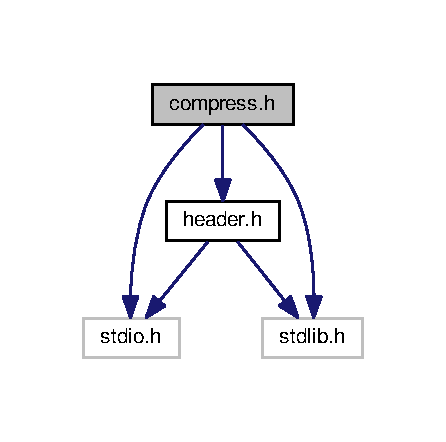
\includegraphics[width=214pt]{compress_8h__incl}
\end{center}
\end{figure}
Ce graphe montre quels fichiers incluent directement ou indirectement ce fichier \+:
\nopagebreak
\begin{figure}[H]
\begin{center}
\leavevmode
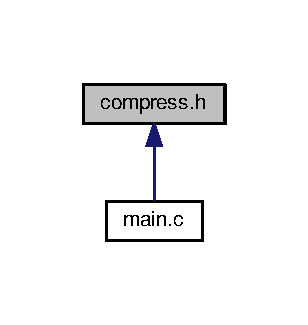
\includegraphics[width=148pt]{compress_8h__dep__incl}
\end{center}
\end{figure}
\subsection*{Fonctions}
\begin{DoxyCompactItemize}
\item 
void \hyperlink{compress_8h_a762f5db62cb619ebc3df5970a4a73404}{compression} (F\+I\+LE $\ast$input, F\+I\+LE $\ast$output, \hyperlink{structCode}{Code} $\ast$codes)
\end{DoxyCompactItemize}


\subsection{Description détaillée}
\begin{DoxyAuthor}{Auteur}
Hareski 
\end{DoxyAuthor}
\begin{DoxyVersion}{Version}
1.\+1 
\end{DoxyVersion}
\begin{DoxyDate}{Date}
16 décembre 2017 
\end{DoxyDate}


\subsection{Documentation des fonctions}
\mbox{\Hypertarget{compress_8h_a762f5db62cb619ebc3df5970a4a73404}\label{compress_8h_a762f5db62cb619ebc3df5970a4a73404}} 
\index{compress.\+h@{compress.\+h}!compression@{compression}}
\index{compression@{compression}!compress.\+h@{compress.\+h}}
\subsubsection{\texorpdfstring{compression()}{compression()}}
{\footnotesize\ttfamily void compression (\begin{DoxyParamCaption}\item[{F\+I\+LE $\ast$}]{input,  }\item[{F\+I\+LE $\ast$}]{output,  }\item[{\hyperlink{structCode}{Code} $\ast$}]{codes }\end{DoxyParamCaption})}



Fonction de compilation Huffman. 


\begin{DoxyParams}{Paramètres}
{\em input} & F\+I\+L\+E$\ast$\+: fichier à analyser au niveau de l\textquotesingle{}encodage \\
\hline
{\em output} & F\+I\+L\+E$\ast$\+: fichier pour la compression \\
\hline
{\em codes} & Code$\ast$\+: codage des caractéres A\+S\+C\+II \\
\hline
\end{DoxyParams}
\begin{DoxyReturn}{Renvoie}
void 
\end{DoxyReturn}

\hypertarget{decompress_8h}{}\section{Référence du fichier decompress.\+h}
\label{decompress_8h}\index{decompress.\+h@{decompress.\+h}}
{\ttfamily \#include $<$stdio.\+h$>$}\newline
{\ttfamily \#include $<$stdlib.\+h$>$}\newline
{\ttfamily \#include \char`\"{}header.\+h\char`\"{}}\newline
Graphe des dépendances par inclusion de decompress.\+h\+:
\nopagebreak
\begin{figure}[H]
\begin{center}
\leavevmode
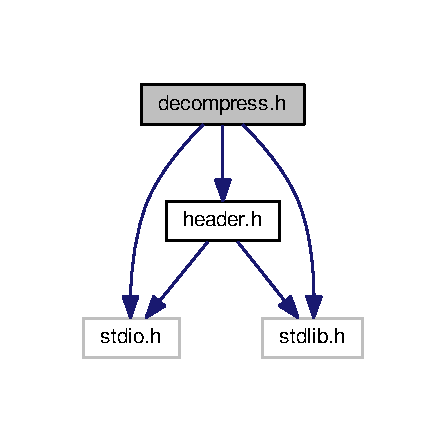
\includegraphics[width=214pt]{decompress_8h__incl}
\end{center}
\end{figure}
Ce graphe montre quels fichiers incluent directement ou indirectement ce fichier \+:
\nopagebreak
\begin{figure}[H]
\begin{center}
\leavevmode
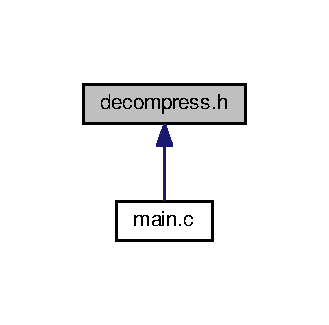
\includegraphics[width=158pt]{decompress_8h__dep__incl}
\end{center}
\end{figure}
\subsection*{Fonctions}
\begin{DoxyCompactItemize}
\item 
void \hyperlink{decompress_8h_a3a294ccb5178e29b844001f7e04a078b}{decompression} (F\+I\+LE $\ast$input, F\+I\+LE $\ast$output, \hyperlink{structNoeud}{Noeud} $\ast$\hyperlink{header_8h_a755eccf14aa051a856c91938297836cd}{tableau\+Huffmann}, int nbr\+Char, int nbr\+A\+S\+C\+II)
\end{DoxyCompactItemize}


\subsection{Description détaillée}
\begin{DoxyAuthor}{Auteur}
Hareski 
\end{DoxyAuthor}
\begin{DoxyVersion}{Version}
1.\+1 
\end{DoxyVersion}
\begin{DoxyDate}{Date}
16 décembre 2017 
\end{DoxyDate}


\subsection{Documentation des fonctions}
\mbox{\Hypertarget{decompress_8h_a3a294ccb5178e29b844001f7e04a078b}\label{decompress_8h_a3a294ccb5178e29b844001f7e04a078b}} 
\index{decompress.\+h@{decompress.\+h}!decompression@{decompression}}
\index{decompression@{decompression}!decompress.\+h@{decompress.\+h}}
\subsubsection{\texorpdfstring{decompression()}{decompression()}}
{\footnotesize\ttfamily void decompression (\begin{DoxyParamCaption}\item[{F\+I\+LE $\ast$}]{input,  }\item[{F\+I\+LE $\ast$}]{output,  }\item[{\hyperlink{structNoeud}{Noeud} $\ast$}]{tableau\+Huffmann,  }\item[{int}]{nbr\+Char,  }\item[{int}]{nbr\+A\+S\+C\+II }\end{DoxyParamCaption})}



Fonction de décompilation Huffman. 


\begin{DoxyParams}{Paramètres}
{\em input} & F\+I\+L\+E$\ast$\+: fichier à analyser au niveau de l\textquotesingle{}encodage \\
\hline
{\em output} & F\+I\+L\+E$\ast$\+: fichier pour l\textquotesingle{}extraction \\
\hline
{\em tableau\+Huffmann} & Noeud$\ast$ \+: tableau de Huffmann de l\textquotesingle{}index \\
\hline
{\em nbr\+Char} & int\+: nombre de caractéres dans input \\
\hline
\end{DoxyParams}
\begin{DoxyReturn}{Renvoie}
void 
\end{DoxyReturn}

\hypertarget{header_8h}{}\section{Référence du fichier header.\+h}
\label{header_8h}\index{header.\+h@{header.\+h}}
{\ttfamily \#include $<$stdio.\+h$>$}\newline
{\ttfamily \#include $<$stdlib.\+h$>$}\newline
Graphe des dépendances par inclusion de header.\+h\+:
\nopagebreak
\begin{figure}[H]
\begin{center}
\leavevmode
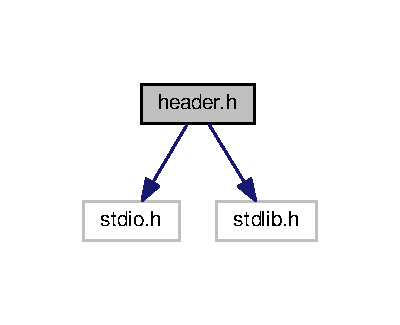
\includegraphics[width=192pt]{header_8h__incl}
\end{center}
\end{figure}
Ce graphe montre quels fichiers incluent directement ou indirectement ce fichier \+:
\nopagebreak
\begin{figure}[H]
\begin{center}
\leavevmode
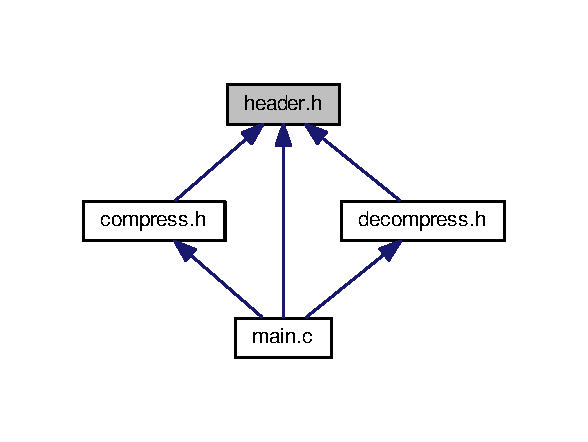
\includegraphics[width=282pt]{header_8h__dep__incl}
\end{center}
\end{figure}
\subsection*{Classes}
\begin{DoxyCompactItemize}
\item 
struct \hyperlink{structNoeud}{Noeud}
\item 
struct \hyperlink{structCode}{Code}
\end{DoxyCompactItemize}
\subsection*{Fonctions}
\begin{DoxyCompactItemize}
\item 
double $\ast$ \hyperlink{header_8h_a523c34b2f1368e288d98a5ad75136bd0}{frequency} (F\+I\+LE $\ast$input, int $\ast$nbr\+Char, int $\ast$nbr\+A\+S\+C\+II)
\item 
\hyperlink{structNoeud}{Noeud} $\ast$ \hyperlink{header_8h_a755eccf14aa051a856c91938297836cd}{tableau\+Huffmann} (double $\ast$freq\+Ascii)
\item 
\hyperlink{structCode}{Code} $\ast$ \hyperlink{header_8h_a8b873c7b4f8fc2bbcfe39c1f862cefde}{save\+Header} (F\+I\+LE $\ast$output, \hyperlink{structNoeud}{Noeud} $\ast$\hyperlink{header_8h_a755eccf14aa051a856c91938297836cd}{tableau\+Huffmann}, int nbr\+Char, int nbr\+A\+S\+C\+II)
\item 
\hyperlink{structNoeud}{Noeud} $\ast$ \hyperlink{header_8h_ab317cd8d11bcc3efa9ee09b26766313e}{get\+Header} (F\+I\+LE $\ast$input, int $\ast$nbr\+Char, int $\ast$nbr\+A\+S\+C\+II)
\end{DoxyCompactItemize}


\subsection{Description détaillée}
\begin{DoxyAuthor}{Auteur}
Hareski 
\end{DoxyAuthor}
\begin{DoxyVersion}{Version}
1.\+1 
\end{DoxyVersion}
\begin{DoxyDate}{Date}
16 décembre 2017 
\end{DoxyDate}


\subsection{Documentation des fonctions}
\mbox{\Hypertarget{header_8h_a523c34b2f1368e288d98a5ad75136bd0}\label{header_8h_a523c34b2f1368e288d98a5ad75136bd0}} 
\index{header.\+h@{header.\+h}!frequency@{frequency}}
\index{frequency@{frequency}!header.\+h@{header.\+h}}
\subsubsection{\texorpdfstring{frequency()}{frequency()}}
{\footnotesize\ttfamily double$\ast$ frequency (\begin{DoxyParamCaption}\item[{F\+I\+LE $\ast$}]{input,  }\item[{int $\ast$}]{nbr\+Char,  }\item[{int $\ast$}]{nbr\+A\+S\+C\+II }\end{DoxyParamCaption})}



Fonction de calcul de la fréquences d\textquotesingle{}A\+S\+C\+II Etendu. 


\begin{DoxyParams}{Paramètres}
{\em input} & F\+I\+L\+E$\ast$\+: fichier à analyser \\
\hline
{\em nbr\+Char} & int\&\+: nombre de caractéres dans input \\
\hline
{\em nbr\+A\+S\+C\+II} & int\&\+: nombre de caractéres distinct dans input \\
\hline
\end{DoxyParams}
\begin{DoxyReturn}{Renvoie}
void 
\end{DoxyReturn}
\mbox{\Hypertarget{header_8h_ab317cd8d11bcc3efa9ee09b26766313e}\label{header_8h_ab317cd8d11bcc3efa9ee09b26766313e}} 
\index{header.\+h@{header.\+h}!get\+Header@{get\+Header}}
\index{get\+Header@{get\+Header}!header.\+h@{header.\+h}}
\subsubsection{\texorpdfstring{get\+Header()}{getHeader()}}
{\footnotesize\ttfamily \hyperlink{structNoeud}{Noeud}$\ast$ get\+Header (\begin{DoxyParamCaption}\item[{F\+I\+LE $\ast$}]{input,  }\item[{int $\ast$}]{nbr\+Char,  }\item[{int $\ast$}]{nbr\+A\+S\+C\+II }\end{DoxyParamCaption})}



Fonction de récupération sur fichier d\textquotesingle{}arbre Huffman. 


\begin{DoxyParams}{Paramètres}
{\em input} & F\+I\+L\+E$\ast$\+: fichier de l\textquotesingle{}index \\
\hline
{\em nbr\+Char} & int$\ast$\+: nombre de caractéres dans input \\
\hline
{\em nbr\+A\+S\+C\+II} & int$\ast$\+: nombre de A\+S\+C\+II distinct \\
\hline
\end{DoxyParams}
\begin{DoxyReturn}{Renvoie}
Noeud$\ast$ \+: tableau d\textquotesingle{}Huffmann 
\end{DoxyReturn}
\mbox{\Hypertarget{header_8h_a8b873c7b4f8fc2bbcfe39c1f862cefde}\label{header_8h_a8b873c7b4f8fc2bbcfe39c1f862cefde}} 
\index{header.\+h@{header.\+h}!save\+Header@{save\+Header}}
\index{save\+Header@{save\+Header}!header.\+h@{header.\+h}}
\subsubsection{\texorpdfstring{save\+Header()}{saveHeader()}}
{\footnotesize\ttfamily \hyperlink{structCode}{Code}$\ast$ save\+Header (\begin{DoxyParamCaption}\item[{F\+I\+LE $\ast$}]{output,  }\item[{\hyperlink{structNoeud}{Noeud} $\ast$}]{tableau\+Huffmann,  }\item[{int}]{nbr\+Char,  }\item[{int}]{nbr\+A\+S\+C\+II }\end{DoxyParamCaption})}



Fonction de sauvegarde fichier et tableau d\textquotesingle{}arbre Huffman. 


\begin{DoxyParams}{Paramètres}
{\em output} & F\+I\+L\+E$\ast$\+: fichier pour l\textquotesingle{}index \\
\hline
{\em tableau\+Huffmann} & Noeud$\ast$ \+: tableau de Huffmann de l\textquotesingle{}index \\
\hline
{\em nbr\+Char} & int\+: nombre de caractéres dans input \\
\hline
{\em nbr\+A\+S\+C\+II} & int\+: nombre de A\+S\+C\+II distinct \\
\hline
\end{DoxyParams}
\begin{DoxyReturn}{Renvoie}
Code$\ast$ \+: tableau des codes A\+S\+C\+II selon l\textquotesingle{}arbre 
\end{DoxyReturn}
\mbox{\Hypertarget{header_8h_a755eccf14aa051a856c91938297836cd}\label{header_8h_a755eccf14aa051a856c91938297836cd}} 
\index{header.\+h@{header.\+h}!tableau\+Huffmann@{tableau\+Huffmann}}
\index{tableau\+Huffmann@{tableau\+Huffmann}!header.\+h@{header.\+h}}
\subsubsection{\texorpdfstring{tableau\+Huffmann()}{tableauHuffmann()}}
{\footnotesize\ttfamily \hyperlink{structNoeud}{Noeud}$\ast$ tableau\+Huffmann (\begin{DoxyParamCaption}\item[{double $\ast$}]{freq\+Ascii }\end{DoxyParamCaption})}



Fonction de géneration d\textquotesingle{}arbre Huffman. 


\begin{DoxyParams}{Paramètres}
{\em tab\+A\+S\+C\+II} & double$\ast$ \+: frequences de chaque codage A\+S\+C\+II \\
\hline
\end{DoxyParams}
\begin{DoxyReturn}{Renvoie}
Noeud$\ast$ \+: arbre de compression et décompression 
\end{DoxyReturn}

\hypertarget{main_8c}{}\section{Référence du fichier main.\+c}
\label{main_8c}\index{main.\+c@{main.\+c}}
{\ttfamily \#include $<$string.\+h$>$}\newline
{\ttfamily \#include $<$stdio.\+h$>$}\newline
{\ttfamily \#include $<$stdlib.\+h$>$}\newline
{\ttfamily \#include \char`\"{}header.\+h\char`\"{}}\newline
{\ttfamily \#include \char`\"{}compress.\+h\char`\"{}}\newline
{\ttfamily \#include \char`\"{}decompress.\+h\char`\"{}}\newline
Graphe des dépendances par inclusion de main.\+c\+:
\nopagebreak
\begin{figure}[H]
\begin{center}
\leavevmode
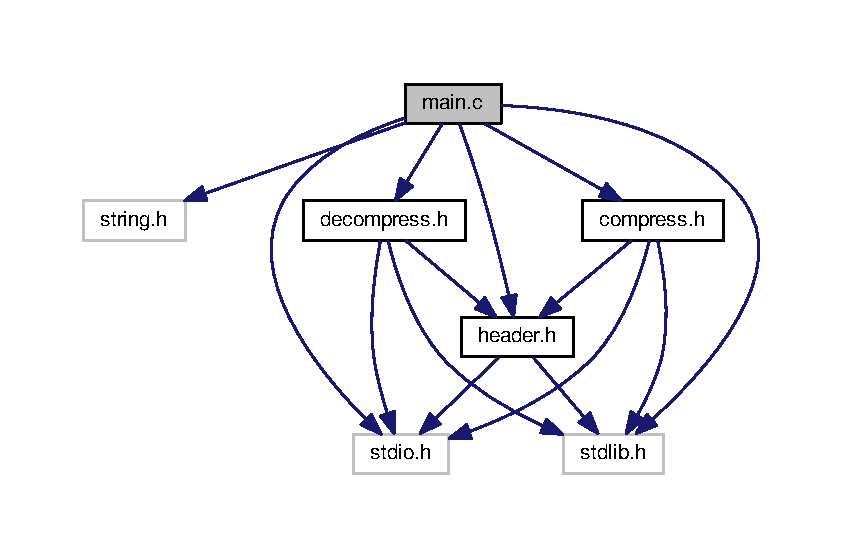
\includegraphics[width=350pt]{main_8c__incl}
\end{center}
\end{figure}
\subsection*{Fonctions}
\begin{DoxyCompactItemize}
\item 
void \hyperlink{main_8c_a57626e1ad092eac4ee80fa406ae0bf6d}{help} (char $\ast$exe\+Name)
\item 
int \hyperlink{main_8c_a0ddf1224851353fc92bfbff6f499fa97}{main} (int argc, char $\ast$argv\mbox{[}$\,$\mbox{]})
\end{DoxyCompactItemize}


\subsection{Description détaillée}
\begin{DoxyAuthor}{Auteur}
Hareski 
\end{DoxyAuthor}
\begin{DoxyVersion}{Version}
1.\+1 
\end{DoxyVersion}
\begin{DoxyDate}{Date}
16 décembre 2017 
\end{DoxyDate}


\subsection{Documentation des fonctions}
\mbox{\Hypertarget{main_8c_a57626e1ad092eac4ee80fa406ae0bf6d}\label{main_8c_a57626e1ad092eac4ee80fa406ae0bf6d}} 
\index{main.\+c@{main.\+c}!help@{help}}
\index{help@{help}!main.\+c@{main.\+c}}
\subsubsection{\texorpdfstring{help()}{help()}}
{\footnotesize\ttfamily void help (\begin{DoxyParamCaption}\item[{char $\ast$}]{exe\+Name }\end{DoxyParamCaption})}



Affiche l\textquotesingle{}aide. 


\begin{DoxyParams}{Paramètres}
{\em exe\+Name} & char$\ast$\+: nom de l\textquotesingle{}executable \\
\hline
\end{DoxyParams}
\begin{DoxyReturn}{Renvoie}
void 
\end{DoxyReturn}
\mbox{\Hypertarget{main_8c_a0ddf1224851353fc92bfbff6f499fa97}\label{main_8c_a0ddf1224851353fc92bfbff6f499fa97}} 
\index{main.\+c@{main.\+c}!main@{main}}
\index{main@{main}!main.\+c@{main.\+c}}
\subsubsection{\texorpdfstring{main()}{main()}}
{\footnotesize\ttfamily int main (\begin{DoxyParamCaption}\item[{int}]{argc,  }\item[{char $\ast$}]{argv\mbox{[}$\,$\mbox{]} }\end{DoxyParamCaption})}



Entrée du programme. 


\begin{DoxyParams}{Paramètres}
{\em argc} & int\+: nombre de paramétres \\
\hline
{\em argv} & char$\ast$$\ast$\+: paramétres \\
\hline
\end{DoxyParams}
\begin{DoxyReturn}{Renvoie}
0\mbox{[}Arrêt normal du programme\mbox{]} ou int\mbox{[}Numéro erreur\mbox{]} 
\end{DoxyReturn}

%--- End generated contents ---

% Index
\backmatter
\newpage
\phantomsection
\clearemptydoublepage
\addcontentsline{toc}{chapter}{Index}
\printindex

\end{document}
